% !TeX root = ../main.tex
% Add the above to each chapter to make compiling the PDF easier in some editors.

\chapter{Baum-Welch Implementation}\label{chapter:hmm-impl}

One of the functionalities of the time series generation tool implemented for this thesis is generating time series using Hidden Markov Models. Specifically you are able to specify training time series to learn HMM parameters to then generate time series from. The learning problem is of course solved using the Baum Welch algorithm, which the tool implements. In this section we will look at the Python implementation of Baum-Welch within the time series generation tool. \parencite{tsgenerator}

\section{fit() Function}

\begin{figure}
\begin{singlespace}
\begin{lstlisting}[language=Python]
def fit(A, k, it):
    means, cov, startprop, transmat = init(k, A)
    for i in range(it):
        e_sumgamma = np.zeros(k)
        e_xgammasum = np.zeros(k)
        e_xgammasumsquared = np.zeros(k)
        e_start = np.zeros(k)
        e_trans = np.zeros((k, k))
        prop = 0
        for X in A:
            n = len(X)
            loglikelihood = log_likelihood(X, k, means, cov)

            logalpha = forward(loglikelihood, startprop, transmat)
            prop += logsumexp(logalpha[-1])

            logbeta = backward(loglikelihood, transmat)

            loggamma = logalpha + logbeta
            gamma = lognormalize_gamma(loggamma)

            e_start += gamma[0]
            e_sumgamma += np.einsum("ij->j", gamma)
            e_xgammasum += np.dot(gamma.T, X)
            e_xgammasumsquared += np.dot(gamma.T, X**2)
            if n > 1:
                logtrans = compute_trans(logalpha, logbeta, \
                    loglikelihood, transmat)
                e_trans += np.exp(logtrans)

        startprop, transmat, means, cov = update_params(e_sumgamma, \
            e_xgammasum, e_xgammasumsquared, e_start, e_trans)
    return startprop, transmat, means, cov
\end{lstlisting}
\end{singlespace}
   
\caption{HMM fit function}    
\label{fig:hmm-fit-listing}
\end{figure}

Figure \ref{fig:hmm-fit-listing} shows the code of the fit function, which is the high level function implementing the parameter learning for HMMs. It takes the parameters A, k, and "it". A is an array of time series, which are the training data. k is the number of hidden states in the HMM. And "it" is the number of iterations of the Baum-Welch algorithm that will be run. 

The function returns the learned parameters "startprop", "transmat", "means", and "cov". "startprop" represents the start probabilities $\pi$, while "transmat" are the transition probabilities $a$. This implementation is a semi-continuos HMM, which means that the emission probabilities take the form of $\mu$ and $\sigma$, which are returned as "means" and "cov". 

In line 2 the parameters get initialized. We will look at the initialization strategy in detail later. Then follows the main loop which applies the EM algorithm to the parameters the specified number of times. 

The first part of the EM-algorithm implementation initializes variables starting with e signifying that they are part of the E-step. Then the inner loop at line 10 applies the Baum-Welch steps to each of the time series in the training set A. First the forward and backwards algorithm are applied to obtain alpha and beta. Both rely on the likelihood, which is computed first then passed in to both functions. 

Note that the implementation differs from the theory here. Instead of computing the intermediate values alpha and beta their log is computed. This is done for accuracy. Since the probabilities can get very low there is the risc of underflow, so they are better represented as logs. Only in the very last step, when computing gamma and trans (which is the sum of xi), do we go back to the regular space from log-space. 

The results for each of the training time series get accumulated in the e variables. Since the M-step involves normalization, simply adding them together works. In the case of "e-trans", which will be used in the M-step to compute the new transition probabilities, it only receives contributions from time series longer then 1. Time series with only a single data point do not give any information about transitions.

Finally using the accumulated data from all training time series in the E-step "update\_params" performs the M-step and returns new values for the four parameters "startprop", "transprop", "means", and "cov". 

\section{Log Likelihood}

From Equation \eqref{eq:prop-statement} we know that the probability of a time series given current parameters can be computed by summing up the last row of $\alpha$. This is whats happening in line 15 in Figure \ref{fig:hmm-fit-listing}. Since we are in log space we add together the probabilities of the individual training time series instead of multiplying them.

\begin{figure}
   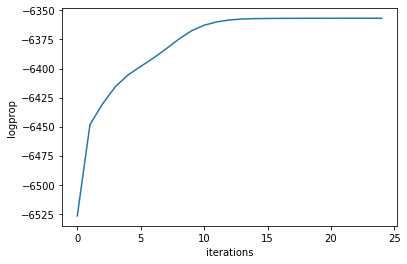
\includegraphics{figures/logprop.png}
   \caption{Logprop during training}
      
   \label{fig:lopprop-graph}
\end{figure}

Figure \ref{fig:lopprop-graph} shows an example of the progression of the log probability during training. The graph is strictly increasing showing that each iteration of the EM-algorithm brings us closer to the optimal values for the parameters. Note that the values are extremely small with their log being less than -6000. This shows that it is necessary to do these computations in log space, the values would get to small otherwise. 

The probability converges relatively quickly, In this case after 10 iterations. After that the change is not noticeable anymore. This implementation works by specifying a number of iterations. However a different system based on monitoring the log probability is also possible. After each iteration check if the change in probability is significant. If not we are converged and the learning is stopped.

\section{init() Function}

\begin{figure}
\begin{singlespace}
\begin{lstlisting}[language=Python]
def init(components, X):
    # join sequences if necessary
    if X.ndim == 2:
        X = np.concatenate(X)
    # initial means using kmeans
    kmeans = sklearn.cluster.KMeans(n_clusters=components)
    kmeans.fit(X.reshape(-1, 1))
    means = kmeans.cluster_centers_.reshape(-1)

    # initial covariance
    covar = np.cov(X)
    cov = np.tile(covar, components)
    # init start probability
    startprop = np.tile(1/components, components)
    # init transition matrix
    transmat = np.tile(1/components, components **
                       2).reshape(components, components)
    return means, cov, startprop, transmat
\end{lstlisting}
\end{singlespace}
   
\caption{HMM init function}    
\label{fig:hmm-init-listing}
\end{figure}

As mentioned before, while we know that EM-algorithms will converge to a maximum, we are not guaranteed to end up at the global maximum. To avoid getting stuck in local maxima the initial values for the parameters are important. They are picked by the init function shown in Figure \ref{fig:hmm-init-listing}

Since we are in a semi-continuos HMM the parameters that have to be initialized are $\pi$, $a$, $\mu$, and $\sigma$, or as they are called in code startprop, transmat, means, and cov. The parameters to the function are the number of hidden states "components" and the training data X, which is either one or multiple time series. The function returns the four initialized parameters. 

The means are initialized by running the k-means algorithm on the training data with the number of hidden states of the HMM as the number of clusters k. K-means is an excellent choice for initializing this since we are assuming that the data is generated by k hidden states, which leads to k clusters of data points. 

All the implementations in the time-series generation tool are done from scratch only using numpy as a dependency. This is the one exception: we use the k-means implementation from sklearn. \parencite{pedregosa2011scikit}  This is because this part is not essential to the Baum-Welch algorithm and it would add a lot of code to implement this from scratch also. Interestingly the k-means algorithm as also an EM-algorithm just as Baum-Welch is. 

The variances are initialized to be the covariance of the training data. In case there are multiple training time-series they are concatenated and the covariance of the concatenation is used. "cov" is a vector of length k, k being the number of hidden states. All entries of the vector receive the same initial value. 

"statprop" and "transmat" are just initialized to have evenly distributed probabilities. For example with four hidden states they will look like this: 

\begin{equation}
a = 
\begin{pmatrix}
\frac{1}{4} & \frac{1}{4} & \frac{1}{4} & \frac{1}{4} \\
\frac{1}{4} & \frac{1}{4} & \frac{1}{4} & \frac{1}{4} \\
\frac{1}{4} & \frac{1}{4} & \frac{1}{4} & \frac{1}{4} \\
\frac{1}{4} & \frac{1}{4} & \frac{1}{4} & \frac{1}{4} \\
\end{pmatrix}
\;\;\;\;
\pi = 
\begin{pmatrix}
\frac{1}{4}  \\
\frac{1}{4}  \\
\frac{1}{4}  \\
\frac{1}{4}  \\
\end{pmatrix}
\end{equation}

\section{log\_likelihood Function}

\begin{figure}
\begin{singlespace}
\begin{lstlisting}[language=Python]
def log_normal_pdf(x, mu, sigmasq):
    dsq = (x - mu)**2
    lp = - 0.5 * np.log(sigmasq * 2 * np.pi) - 0.5 * dsq / sigmasq
    return lp


def log_likelihood(X, k, means, cov):
    ll = np.zeros((len(X), k))
    for i in range(len(X)):
        for j in range(k):
            ll[i, j] = log_normal_pdf(X[i], means[j], cov[j])

    return ll
\end{lstlisting}
\end{singlespace}
   
\caption{HMM log\_likelihood function}    
\label{fig:hmm-ll-listing}
\end{figure}

For both the forward and backward algorithm we need the likelihoods of the observed outputs according to the current parameters. This is implemented in the function log\_likelihood shown in Figure \ref{fig:hmm-ll-listing}. The parameters are X the observed time series, k the number of hidden states, means and cov the current parameters for emission probability. The function then computes the likelihood of the observed output at every time point for every hidden state. To compute the likelihood the probability density function of the normal distribution (Equation \eqref{eq:normal-pdf}) is used, specifically the log of that probability. Finally a matrix with all time and hidden state combinations is returned. 

\begin{equation}
  \mathcal{N}\left(\mu, \sigma^{2}\right) = \frac{1}{\sigma \sqrt{2 \pi}} e^{-\frac{1}{2}\left(\frac{x-\mu}{\sigma}\right)^{2}} 
  \label{eq:normal-pdf}
\end{equation}

\section{forward Function}

\begin{figure}
\begin{singlespace}
\begin{lstlisting}[language=Python]
def forward(loglikelihood, start, transition):
    n, k = loglikelihood.shape
    # taking the log of 0 gives -inf, which is fine in this case
    with np.errstate(divide="ignore"):
        logstart = np.log(start)
        logtrans = np.log(transition)
    alpha = np.zeros((n, k))
    temp = np.zeros(k)

    for i in range(k):
        alpha[0, i] = logstart[i] + loglikelihood[0, i]

    for t in range(1, n):
        for j in range(k):
            for i in range(k):
                temp[i] = alpha[t-1, i] + logtrans[i, j]
            alpha[t, j] = logsumexp(temp) + loglikelihood[t, j]
    return alpha
\end{lstlisting}
\end{singlespace}
   
\caption{HMM forward function}    
\label{fig:hmm-forward-listing}
\end{figure}

Figure \ref{fig:hmm-forward-listing} shows the implementation of the forward algorithm. It takes as parameters the previously computed loglikelihood, and the current HMM parameters start and transition or $\pi$  and $a$. The implementation follows the recursive definition of $\alpha$ from Equation \eqref{eq:alpha-def}. The first row of alpha is computed using start probability and emission probability, in form of the loglikelihood. Then the remaining rows are each computed based on the previous row. Finally alpha is returned in matrix form. 

The notable differences to the theoretical formulas are that we are again in log-space. We take the log of the parameters start and transition at the beginning. "loglikelihood" obviously is in log-space already. When trying to take the log of 0 Python will return "-inf" and show a warning. This warning is disabled since this is the desired behavior. Being in log-space also turns all the multiplications in the definition of alpha to additions. However there is also a sum in the recursive part of the alpha definition. This gets computed with the help of the logsumexp function. 

\section{logsumexp Function}

\begin{figure}
\begin{singlespace}
\begin{lstlisting}[language=Python]
def logsumexp(ns):
    max = np.max(ns)
    # negative inf case
    if np.isneginf(max):
        return float("-inf")
    ds = ns - max
    sumOfExp = np.exp(ds).sum()
    return max + np.log(sumOfExp)

\end{lstlisting}
\end{singlespace}
\caption{logsumexp function}    
\label{fig:logsumexp-listing}
\end{figure}

In Machine Learning in general we often have to compute equations of this form: 

\begin{equation}
y=\log \sum_{i=1}^{n} e^{x_{i}}
\end{equation}

As is the case in out forward algorithm code among other places in the Baum-Welch algorithm. We are in log-space but we want to take a sim in regular space. The solution is to exponentiate every part of the sum, do the addition, and finally take the log again. The issue here is that we loose the numerical advantages that we gained by operating in log-space in the first place. The solution to this problem can be found in this property:

\begin{equation}
\log \sum_{i=1}^{n} e^{x_{i}}=a+\log \sum_{i=1}^{n} e^{x_{i}-a}
\end{equation}

Suppose all of the $e^{x_i}$ are very large but close together. Then by choosing a appropriate $a$ we can compute the sum of the smaller $e^{x_i-a}$ then make up the difference in log space by adding a again. This avoids inaccuracies. A reasonable choice for a is the maximum value of the sum. This is the approach taken in the logsumexp implementation in line 2. There is the edge case of one part of the sum being negative infinity, which will lead to the whole sum evaluating to negative infinity. \parencite{mllecture}

\section{backwards Function}

The backwards function computes $\beta$ according to its definition in Equation \ref{eq:beta-def}. Its implementation is shown in Figure \ref{fig:hmm-backwards-listing}. The consideration are essentially the same as for the forward algorithm. 

\begin{figure}
\begin{singlespace}
\begin{lstlisting}[language=Python]
def backward(loglikelihood, transition):
   n, k = loglikelihood.shape
   # taking the log of 0 gives -inf, which is fine in this case
   with np.errstate(divide="ignore"):
      logtrans = np.log(transition)
   beta = np.zeros((n, k))
   temp = np.zeros(k)

   for i in range(k):
      beta[-1, i] = 0.0

   for t in range(n-2, -1, -1):
      for i in range(k):
         for j in range(k):
            temp[j] = logtrans[i, j] + loglikelihood[t+1, j] \
                + beta[t+1, j]
         beta[t, i] = logsumexp(temp)
   return beta
\end{lstlisting}
\end{singlespace}
\caption{HMM backwards function}    
\label{fig:hmm-backwards-listing}
\end{figure}

\section{E-step}

The E-step of the Baum-Welch algorithm involves computing the intermediate values $\gamma$ and $\xi$. 

We have already seen the computation of $\gamma$ in the "fit" function in Figure \ref{fig:hmm-fit-listing} in line 19 and 20. $\gamma$ is the product of the previously computed $\alpha$ and $\beta$. Since we are in log space the multiplication turns into an addition. Then $\gamma$ gets normalized using the "lognormalize\_gamma" function seen in Figure \ref{fig:lognormalize-listing}

\begin{figure}
\begin{singlespace}
\begin{lstlisting}[language=Python]
   def lognormalize_gamma(g):
    l = g.shape[0]
    a = np.zeros(l)

    for i in range(l):
        a[i] = logsumexp(g[i])

    g_norm = g - a.reshape(-1, 1)
    return np.exp(g_norm)
\end{lstlisting}
\end{singlespace}
\caption{lognormalize function}    
\label{fig:lognormalize-listing}
\end{figure}

$\gamma$'s rows need to sum up to 1, so each entry has to be divided by the sum of its respective row. Since we are in log-space this sum is computed using the "logsumexp" function. Also because of the log space the division of the entries turns into a subtraction. The normalized gamma is the final step of this computation, so we can leave log-space. For this the "lognormalize\_gamma" function returns the result exponentiated. 

\begin{figure}
\begin{singlespace}
\begin{lstlisting}[language=Python]
def compute_trans(a, b, ll, transition):
   n, k = ll.shape
   with np.errstate(divide="ignore"):
      logtrans = np.log(transition)
   logxisum = np.full((k, k), float("-inf"))
   denom = logsumexp(a[-1])

   for t in range(n-1):
      for i in range(k):
         for j in range(k):
               logxi = a[t, i] + logtrans[i, j] + \
                  ll[t+1, j] + b[t+1, j] - denom
               logxisum[i, j] = logsumexp([logxisum[i, j], logxi])
   return logxisum
\end{lstlisting}
\end{singlespace}
\caption{HMM compute\_trans function}    
\label{fig:hmm-computetrans-listing}
\end{figure}

The second variable in the E-step is $\xi$. It does not appear directly in the high level "fit" function, rather it is computed implicitly in the "compute\_trans" function seen in Figure \ref{fig:hmm-computetrans-listing}. The function takes in the parameters "a", "b", "ll", "transition". They represent alpha, beta, the current emission probability, and the current transition probability respectively. 

$\xi$ is computed according to the second formula given by the Equation \eqref{eq:xi-def}. That is instead of normalizing the denominator is computed from $\alpha$. Similar to the forward and backward algorithm the multiplications and divisions from the formula turn into additions and subtractions in the implementation, since we are in log-space. We never actually use $\xi$ directly: whenever it appears it is summed up over t. So instead of returning the three dimensional $\xi$ with parameters i,j, and t, the function sums up over t during the computation. The function then returns the two dimensional summed $\xi$ with parameters i and j. This summation once again uses "logsumexp". At this point we have again reached the final step of a computation. This means we leave log-space, which happens in line 28 of the "fit" function in Figure \ref{fig:hmm-fit-listing}. The return value of "compute\_trans" gets exponentiated. 

\section{M-step}

\begin{figure}
\begin{singlespace}
\begin{lstlisting}[language=Python]
def update_params(sumgamma, xgammasum, xgammasumsquared, start, trans):
   norm_trans = normalize(trans, axis=1)
   norm_start = normalize(start)

   means = xgammasum / sumgamma
   # cov is based on newly computed means
   num = (means**2 * sumgamma - 2 * means *
         xgammasum + xgammasumsquared)

   cov = (num + 0.01) / np.maximum(sumgamma, 1e-5)

   return norm_start, norm_trans, means, cov
\end{lstlisting}
\end{singlespace}
\caption{HMM update\_params function}    
\label{fig:hmm-updateparams-listing}
\end{figure}

Having completed the E-step the final operation of the Baum-Welch algorithm is the M-step, finding the new parameters that maximize the likelihood in the current iteration of the model. This is done in the function "update\_params" shown in Figure \ref{fig:hmm-updateparams-listing}.

The function takes in the variables accumulated in the E-step: "sumgamma", \\ "xsumgamma", "xsumgammasquared", "start", and "trans" and it returns the new parameters of the HMM $\pi$, $a$, $\mu$, and $\sigma$ as "norm\_start", "norm\_trans", "means", and "cov". 

The parameters start and trans are already the denominators of the new $\pi$ and $a$. Since these two are defined to add up to one, they just have to be normalized to obtain the new parameters. The remaining parameters are $\gamma$ summed up over its rows and the dot-products of $\gamma$ and $x$ and $\gamma$ and $x^2$. They come in computing the remaining two parameters. 

$\mu$ representing the means of the semi-continuos HMM is is computed according to Equation \eqref{eq:mu-def}. It is the fraction of $x$ dot $\gamma$ over sum of $\gamma$. This makes intuitive sense: for each hidden state the mean is a weighed average of all the data-points with the weight being the likelihood of being in that state at that time point. 

Multiplying out Equation \eqref{eq:sigma-def} defining sigma yields this: 

\begin{equation}
   \sigma_i^2 = \frac{\mu_i^2 \sum_t \gamma_t(i) + \sum_t \gamma_t(i)x_t^2 - 2 \mu_i \sum_t x_t \gamma_t(i)}{\sum_t \gamma_t(i)}
\end{equation}

This is what the function uses to compute the final parameter $\sigma$. However there is a slight adjustment in the computation. The numerator get slightly increased by 0.01 and the denominator gets a minimum value of 1e-5. This adjustment prevents the entries in $\sigma$ from becoming both to small or to big to big to prevent overfitting. The specific values come from the popular HMM library hmmlearn. \parencite{weiss2019hmmlearn} Formally this can be thought of as putting a prior on doing a Maximum a Posteriori (MAP) estimate instead of a simple Maximum Likelihood Estimate (MLE). Generally adding a prior is done to prevent overfitting. \parencite{gauvain1994maximum}

The M-step is the last piece of the Baum-Welch algorithm. With this we have looked at all the relevant code that the time-series generation tool uses to learn Hidden Markov Model parameters. 